% =====================================================================
%  MR2006B Industrial Automation -- Module 4: Control
%  Assessment 2: Control design in discrete time for autonomous
%  navigation (simulation environment)
%  IEEE conference template (IEEEtran)
%
%  Data: openloop_test01.zip (Canvas). Red text = still to do.
%  Rubric: specification/sampling time (20), model identification with
%  least squares (50), cross-validation (20), conclusions and learning
%  reflection + paper format (10). Keep it under 8 pages.
% =====================================================================
\documentclass[conference]{IEEEtran}
\IEEEoverridecommandlockouts
\usepackage{cite}
\usepackage{amsmath,amssymb,amsfonts}
\usepackage{graphicx}
\usepackage{textcomp}
\usepackage{xcolor}
\usepackage{booktabs}
\usepackage{tikz}
\usetikzlibrary{positioning,arrows.meta,calc}
\usepackage[hidelinks]{hyperref}

\newcommand{\todo}[1]{\textcolor{red}{[TODO: #1]}}
\newcommand{\figfile}[3][\columnwidth]{%
  \IfFileExists{#2}{\includegraphics[width=#1]{#2}}%
  {\fbox{\parbox[c][#3][c]{\dimexpr#1-2\fboxsep-2\fboxrule}{\centering\small
   \textcolor{red}{\texttt{\detokenize{#2}}} missing}}}}

\begin{document}

\title{Discrete-Time Trajectory Tracking Control with Kalman Filter State
Estimation for an Autonomous Vehicle in Simulation\thanks{Assessment 2,
Industrial Automation (MR2006B.602), Module 4: Control, Prof. Juan Carlos
Tud\'on, Tecnol\'ogico de Monterrey, November 2026. Data and code:
\texttt{github.com/DanielHexZen/euromotion-tec}.}}

\author{
\IEEEauthorblockN{Isaac Sebastian Hovmand}
\IEEEauthorblockA{\textit{A01832781} \\ Tecnol\'ogico de Monterrey\\ Monterrey, Mexico}
\and
\IEEEauthorblockN{Thomas Michael Resch}
\IEEEauthorblockA{\textit{A01832776} \\ Tecnol\'ogico de Monterrey\\ Monterrey, Mexico}
\and
\IEEEauthorblockN{Jan Mosler}
\IEEEauthorblockA{\textit{A01833812} \\ Tecnol\'ogico de Monterrey\\ Monterrey, Mexico}
\and
\IEEEauthorblockN{Daniel Appel}
\IEEEauthorblockA{\textit{A01833285} \\ Tecnol\'ogico de Monterrey\\ Monterrey, Mexico}
}

\maketitle
\thispagestyle{plain}
\pagestyle{plain}

\begin{abstract}
\todo{Write last. 150--200 words: goal, vehicle model, identification
with least squares on \texttt{openloop\_test01}, discrete PID design,
Kalman filter, simulation results with key numbers.}
\end{abstract}

\begin{IEEEkeywords}
discrete-time control, PID, Kalman filter, trajectory tracking,
least squares, ARX model, autonomous navigation
\end{IEEEkeywords}

% =====================================================================
\section{Introduction}
% =====================================================================
An autonomous vehicle must follow a reference trajectory
$(x_r, y_r)$. The controller runs on a microcontroller, so it works in
discrete time. The vehicle sensors are noisy, and the position is not
measured directly. This paper designs a discrete-time tracking controller
and a Kalman filter that estimates the position. Both are tested in a
simulation environment built from models identified on open-loop data.

\todo{Motivation, link to the EuroMotion challenge and to Assessment~1,
contributions of this paper, structure of the paper.}

% =====================================================================
\section{System Description}
% =====================================================================

\subsection{Vehicle and Components}
\todo{Vehicle, actuators, sensors (IMU: $\ddot{x}$, $\ddot{y}$), MCU.
Table with the main components. Photo or schematic.}

\subsection{Control Architecture}
Fig.~\ref{fig:loop} shows the closed loop. The reference point is
compared with the estimated position $(\hat{x}, \hat{y})$. This gives a
distance error $e_x$ and a heading error $e_\theta$, with the desired
heading
\begin{equation}
  \theta_r = \operatorname{atan2}(y_r - \hat{y},\; x_r - \hat{x}).
  \label{eq:heading}
\end{equation}
The PID controllers turn the errors into the speed command $v$ and the
steering angle $\delta$. The Kalman filter uses these inputs and the
measured accelerations $\ddot{x}$, $\ddot{y}$ to estimate the position
that closes the loop.

\begin{figure}[t]
\centering
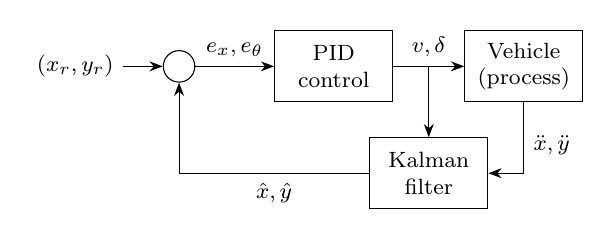
\begin{tikzpicture}[
  >=Stealth, font=\footnotesize, node distance=6mm,
  blk/.style={draw, minimum height=9mm, minimum width=15mm, align=center},
  sum/.style={draw, circle, inner sep=0pt, minimum size=4mm}]
  \node (ref) {$(x_r, y_r)$};
  \node[sum, right=5mm of ref] (s) {};
  \node[blk, right=10mm of s] (pid) {PID\\control};
  \node[blk, right=9mm of pid] (car) {Vehicle\\(process)};
  \node[blk, below=9mm of $(pid)!0.5!(car)$] (kf) {Kalman\\filter};
  \draw[->] (ref) -- (s);
  \draw[->] (s) -- node[above] {$e_x, e_\theta$} (pid);
  \draw[->] (pid) -- node[above] {$v, \delta$} (car);
  \draw[->] ($(pid.east)!0.5!(car.west)$) |- ($(kf.north)+(0,3mm)$) -- (kf.north);
  \draw[->] (car.south) |- node[pos=0.3, right] {$\ddot{x}, \ddot{y}$} (kf.east);
  \draw[->] (kf.west) -| node[pos=0.25, below] {$\hat{x}, \hat{y}$} (s.south);
\end{tikzpicture}
\caption{Closed-loop trajectory tracking with Kalman filter state
estimation.}
\label{fig:loop}
\end{figure}

\subsection{Sampling Time}\label{sec:ts}
\todo{Choose $T_s$ and justify it: dominant time constants from the
identified models, rule of thumb (e.g.\ 5--10 samples per rise time),
sensor rate, MCU load.}

% =====================================================================
\section{Modeling}
% =====================================================================

\subsection{Kinematic Vehicle Model}
\todo{Bicycle model with inputs $v$ and $\delta$:
$\dot{x} = v\cos\theta$, $\dot{y} = v\sin\theta$,
$\dot{\theta} = (v/L)\tan\delta$. Note: nonlinear, linearize or use an
EKF. Map to the differential drive of EuroMotion if needed.}

\subsection{Longitudinal Dynamics}
\todo{Speed response to the command. First-order ARX structure.}

\subsection{Lateral Dynamics}
\todo{Yaw / lateral response to $\delta$. ARX structure.}

% =====================================================================
\section{Identification Method}
% =====================================================================

\subsection{ARX Structure and Least Squares}
\todo{Regression form $y[k] = \varphi^\top[k]\,\vartheta + e[k]$ and the
estimate $\hat{\vartheta} = (\Phi^\top\Phi)^{-1}\Phi^\top Y$.}

\subsection{Data Set}
\todo{Describe \texttt{openloop\_test01}: signals, length, excitation,
pre-processing. At least two tests per dynamic (longitudinal and lateral).}

\subsection{Cross-Validation}
\todo{Train on one data set, validate in free-run simulation on new data
sets. Fit metric (e.g.\ $R^2$, NRMSE).}

% =====================================================================
\section{Controller Design in Discrete Time}
% =====================================================================

\subsection{Discrete PID Controllers}
\todo{Two loops: distance error $\to v$, heading error $\to \delta$.
Discrete PID form, discretization method (Tustin / backward Euler),
tuning method and final gains. Saturation and anti-windup.}

\subsection{Kalman Filter}
The filter uses the linear discrete model
\begin{align}
  x[k+1] &= A\,x[k] + B\,u[k] + w[k], & w &\sim \mathcal{N}(0, Q), \\
  y[k]   &= C\,x[k] + v[k],           & v &\sim \mathcal{N}(0, R),
\end{align}
where $u = [v,\ \delta]^\top$ and $y = [\ddot{x},\ \ddot{y}]^\top$. Each
step has a prediction
\begin{align}
  \hat{x}[k+1|k] &= A\,\hat{x}[k|k] + B\,u[k], \\
  P[k+1|k] &= A\,P[k|k]\,A^\top + Q,
\end{align}
and an update with the new measurement
\begin{align}
  K &= P[k+1|k]\,C^\top \bigl(C\,P[k+1|k]\,C^\top + R\bigr)^{-1}, \\
  \hat{x}[k+1|k+1] &= \hat{x}[k+1|k] + K\bigl(y[k+1] - C\,\hat{x}[k+1|k]\bigr), \\
  P[k+1|k+1] &= (I - K C)\,P[k+1|k].
\end{align}
The filter starts from $\hat{x}[0]$ and $P[0]$.

\todo{State vector, matrices $A$, $B$, $C$, choice of $Q$ and $R$
(e.g.\ $R$ from sensor noise variance in the open-loop data).
Discuss observability: accelerations alone do not fix the absolute
position, so the position estimate relies on the model and drifts.}

% =====================================================================
\section{Simulation Environment}
% =====================================================================
\todo{Tool (MATLAB/Simulink), structure of the simulation, noise
injection, reference trajectories (e.g.\ straight line, circle, double
lane change).}

% =====================================================================
\section{Results}
% =====================================================================

\subsection{Identified Models}
\todo{Table with parameters, time constants, fit on training data.}

\subsection{Cross-Validation}
\todo{Plots and fit on the validation data sets.}

\subsection{Trajectory Tracking}
\todo{Reference vs.\ true vs.\ estimated path. Tracking error (RMS, max).}

\begin{figure}[t]
\centering
\figfile{fig_tracking.pdf}{40mm}
\caption{Reference, true and estimated trajectory.
\todo{generate figure}}
\label{fig:tracking}
\end{figure}

\subsection{Estimation Performance}
\todo{Estimation error with and without the Kalman filter. Effect of
$Q$ and $R$.}

% =====================================================================
\section{Discussion and Limitations}
% =====================================================================
\todo{Model mismatch, drift of the position estimate, nonlinearity,
what would change on the real vehicle.}

% =====================================================================
\section{Conclusions and Learning Reflection}
% =====================================================================
\todo{Main results in a few sentences. What each team member learned.}

\begin{thebibliography}{00}
\bibitem{astrom} K. J. \AA str\"om and B. Wittenmark, \emph{Computer-Controlled
Systems: Theory and Design}, 3rd ed. Mineola, NY, USA: Dover, 2011.
\bibitem{ljung} L. Ljung, \emph{System Identification: Theory for the User},
2nd ed. Upper Saddle River, NJ, USA: Prentice Hall, 1999.
\bibitem{kalman} R. E. Kalman, ``A new approach to linear filtering and
prediction problems,'' \emph{J. Basic Eng.}, vol.~82, no.~1, pp.~35--45, 1960.
\bibitem{rajamani} R. Rajamani, \emph{Vehicle Dynamics and Control}, 2nd ed.
New York, NY, USA: Springer, 2012.
\end{thebibliography}

\end{document}
